% Please use the skeleton file you have received in the
% invitation-to-submit email, where your data are already
% filled in. Otherwise please make sure you insert your
% data according to the instructions in PoSauthmanual.pdf
\documentclass{PoS}

\title{CMS developments for track-triggers}

\ShortTitle{CMS developments for track-triggers}

\author{\speaker{Marco De Mattia}%
        \thanks{For the CMS Collaboration.}\\
       Texas A\&M University\\
       E-mail: \email{marco.de.mattia@cern.ch}}

%\author{Another Author\\
%        Affiliation\\
%        E-mail: \email{...}}

\abstract{The High Luminosity LHC (HL-LHC) is expected to deliver luminosities of 5$\times10^{34}$cm$^{-2}$s$^{-1}$, with an average of about 140 overlapping proton-proton collisions per bunch crossing. These extreme pileup conditions place stringent requirements on the trigger system to be able to cope with the resulting event rates. A key component of the CMS upgrade for HL-LHC is a track trigger system which would identify tracks with transverse momentum above 2 GeV already at the first-level trigger. We present the status of proposals for implementing the L1 tracking in conjunction with the planned upgrade for the silicon tracker of the CMS experiment. The expected performance and the use of L1 tracks for triggering is discussed.}

\FullConference{24th International Workshop on Vertex Detector -VERTEX2015-\\
		1-5 June 2015\\
		Santa Fe, New Mexico, USA}

\begin{document}

\section{Introduction}

The upgrade to the High Luminosity LHC (HL-LHC) is foreseen for Long Shutdown 3 during 2023-2025. The peak luminosity is planned to be 5$\times10^{34}$cm$^{−2}$s$^{−1}$ with a goal to collect 3000 fb$^{−1}$ over a ten year period~\cite{SLHC}. This is predicted to result in an average of 140 overlapping proton-proton collisions per bunch crossing (pileup) posing serious challenges for the LHC experiments. With the HL-LHC, trigger rates at the first-level (L1) trigger for single muons, electrons, and jets would exceed 100 kHz. The key goal for the CMS experiment~\cite{CMS} is to maintain similar physics performance as for the 2012 operation. However, simply increasing the trigger thresholds would restrict the physics potential and would alone not be sufficient. To achieve this goal, a critical component of the upgraded CMS experiment for the HL-LHC is a new tracker with capability to supply data to the L1 trigger processors~\cite{CMSUpgrade}. This would enable the experiment to perform tracking already in the L1 trigger and to maintain high efficiencies and keep event rates under control for L1 trigger objects.

Different approaches are under study for how to perform track finding at the L1 trigger:
\begin{itemize}
\item A so called tracklet-based method~\cite{Tracklet} an algorithmic method which relies on commercial FPGA technology;
\item A method based on FPGA and large time-multiplexing;
\item An approach based on a combination of associative memories (AM)~\cite{AM} and FPGAs.
\end{itemize}
These proceedings describe the basic concepts of the three methods. We also study the expected performance, and illustrates the use of tracks in the L1 trigger.

\section{Track Trigger Concept}

CMS plans to use a self-seeded L1 track trigger which relies on local transverse momentum ($p_T$) reconstruction to enable filtering of hits generated by low $p_T$ tracks. Hits produced by low-$p_T$ tracks are discriminated from those coming from high-$p_T$ tracks utilizing the distance between the hits in the two nearby layers of so called "$p_T$ modules" as illustrated in Figure~\ref{fig:PtModule}. Due to the bending of tracks in the 3.8 T magnetic field of CMS, the distance between the two hits associated with a track provides a measurement of its $p_T$. Correlated pairs of clusters, referred to as stubs, are read out by the trigger if they are pairs of clusters consistent with a track with $p_T \geq$ 2 GeV. This pre-selection is highly powerful as in minimum bias events about 95\% of all tracks have $p_T < $ 2 GeV. The full information is retained in the buffers of the front-end electronics and read out if the event is accepted by the L1 global trigger. The aim is to reconstruct tracks with $p_T >$ 2 GeV and to identify the track z position with $\sim$1 mm precision, similar to the average vertex separation at pileup (PU) of 140.
\begin{figure}[h!]
  \centering
	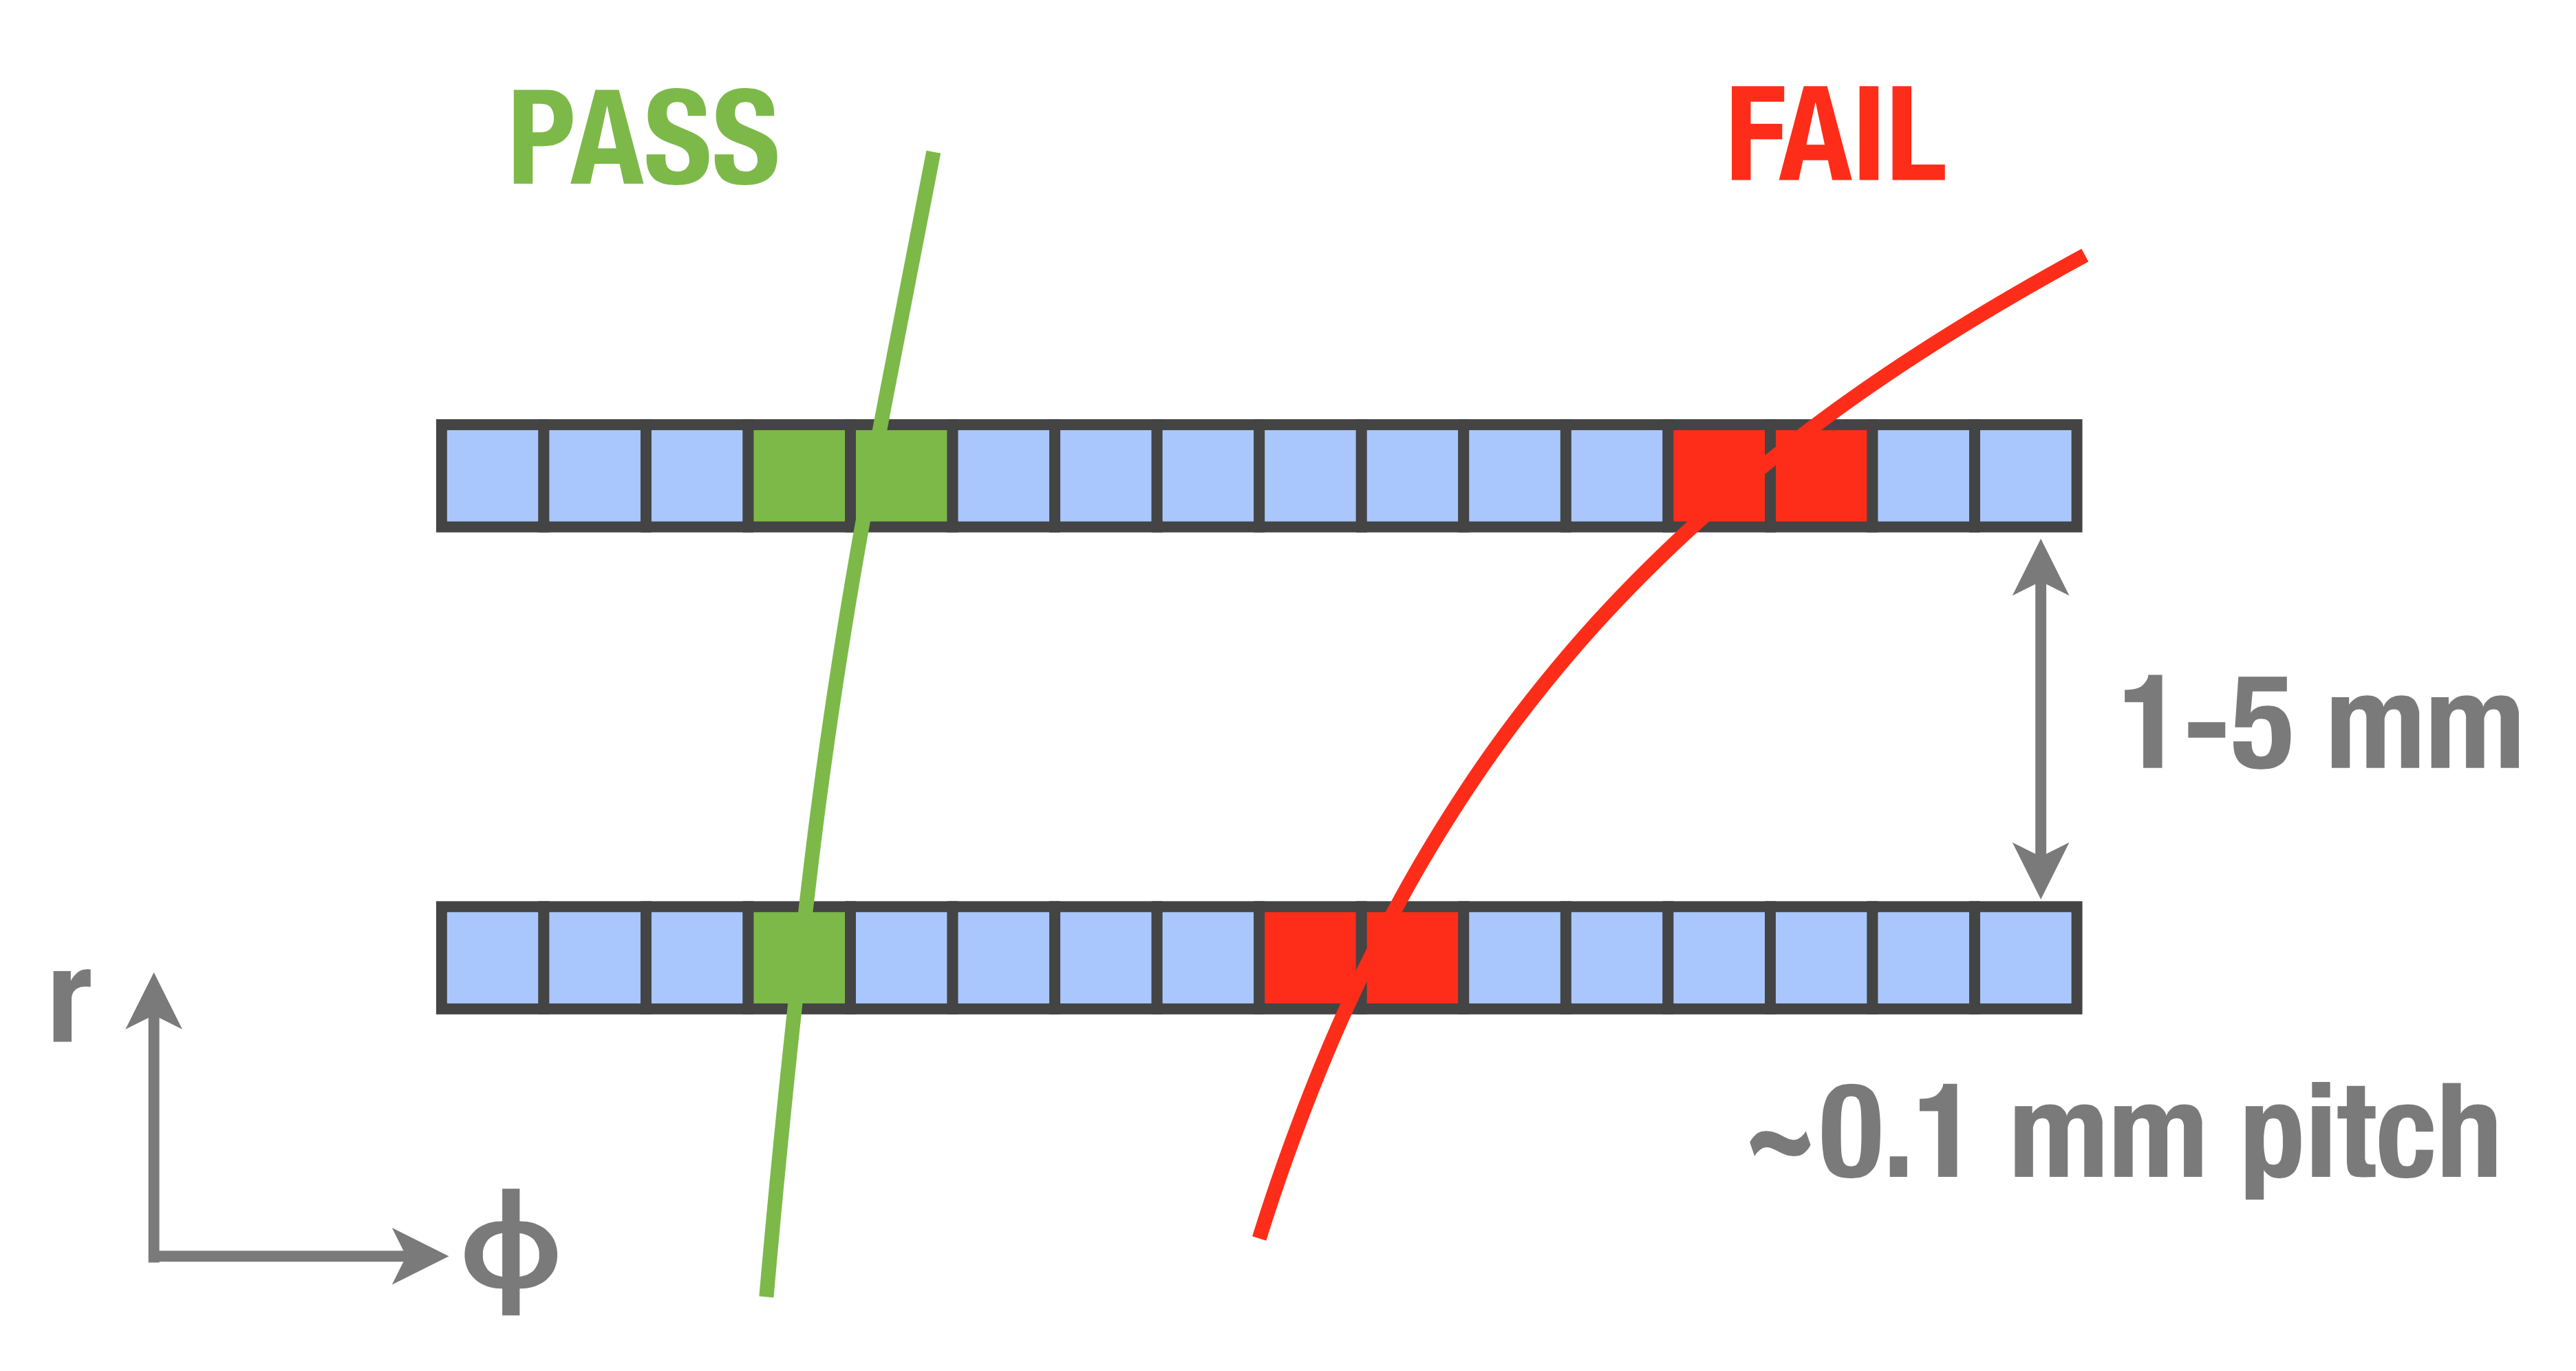
\includegraphics[width=0.5\textwidth]{Figures/PtModule.png}
	\caption{Schematic illustration of stubs passing or failing the momentum discrimination. Trajectories of low-$p_T$ charged particles bend in the magnetic field and produce hits which are not consistent with a high-$p_T$ charged particle coming from the interaction point.}
	\label{fig:PtModule}
\end{figure}

\subsection{Tracker Geometry}

The baseline geometry for the upgraded CMS outer tracker consists of a central barrel with six layers and two endcaps with five disks each. Two types of $p_T$ modules are used: 2S modules in the three outer layers and in the outer rings of the disks, and PS modules in the three inner layers and in the inner rings of the disks. The 2S modules consist of 10 $\times$ 10 cm$^2$ strip sensors: 2 $\times$ 5 cm long strips with 90 $\mu$m pitch. The PS modules have a top sensor with 2 $\times$ 25 mm strips with 100 $\mu$m pitch and a bottom sensor with 1.5 mm $\times$ 100 $\mu$m pixels. Figure~\ref{fig:TrackerLayout} shows the geometry for the outer tracker~\cite{TkLayout}. Also shown is the inner pixel detector which, however, is not utilized in this study.
\begin{figure}[h!]
  \centering
	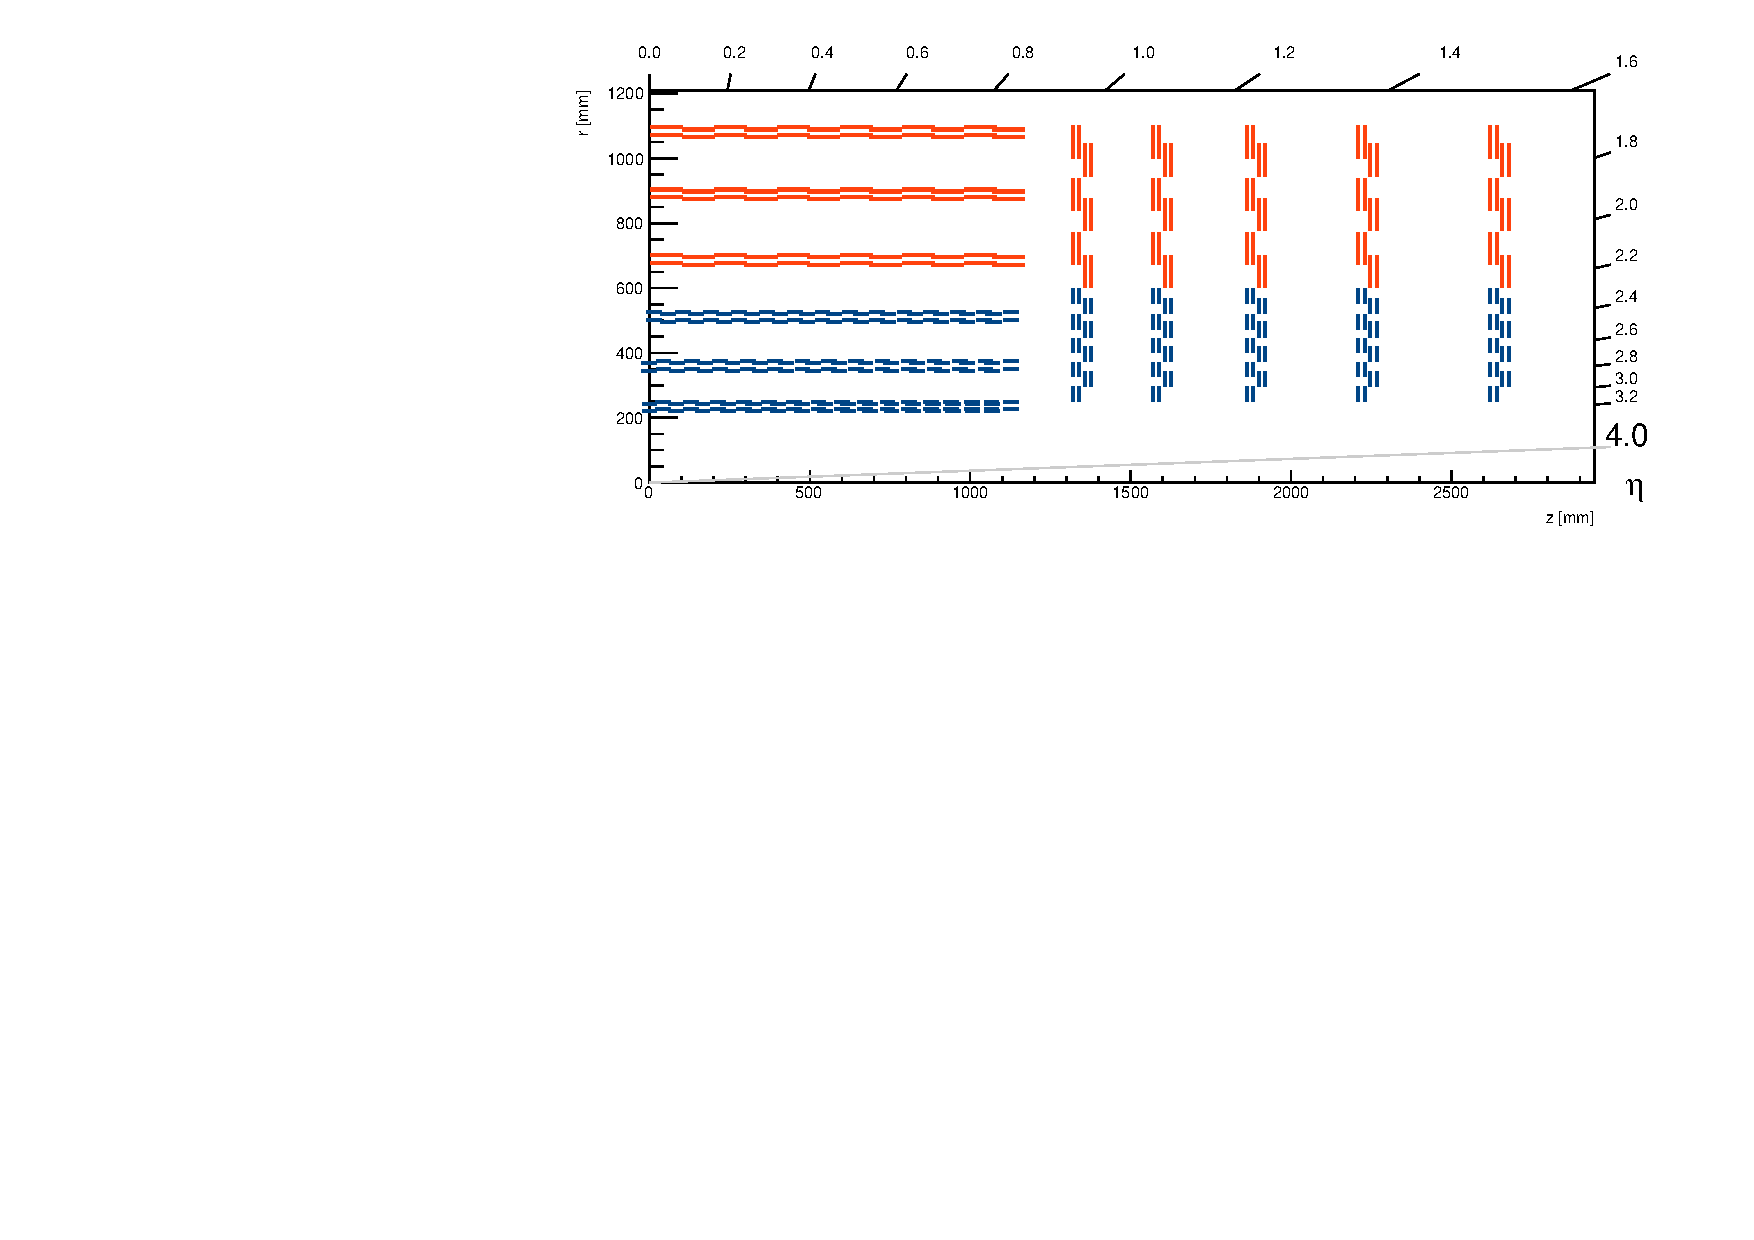
\includegraphics[width=\textwidth]{Figures/TrackerLayout.pdf}
	\caption{Baseline geometry for the upgraded CMS tracker.}
	\label{fig:TrackerLayout}
\end{figure}

\subsection{Tracklet Method for Tracking at L1}

The tracklet-based approach relies on commercial FPGA technology to perform tracking at L1. Track finding is performed in four main steps, starting from the stubs received from the front-end electronics of the tracker. In the first step, tracks are seeded by forming tracklets from pairs of stubs in neighboring layers. A rough estimate of the tracklet parameters is extracted from the two stubs plus a constraint to the beamspot. The tracklet must be consistent with a track with $p_T >$ 2 GeV and a z position $|z_0| <$ 15 cm. To ensure high efficiency the seeding is done multiple times between different layers and disks. Tracklets are then projected, both outside-in and inside-out, to other layers and disks to search for matching stubs. A track fit is performed utilizing all the stubs that are matched to the trajectory of the tracklet. The fit is a linearized $\chi^2$ fit and gives the final track parameters: transverse momentum ($p_T$), pseudorapidity ($\eta$), the azimuthal angle at the point of closest approach in the R-z plane ($\phi_0$), the track z position at the point of closest approach ($z_0$), and optionally the transverse impact parameter ($d_0$). In the following, tracks are constrained to originate from the interaction point in the x-y plane, i.e. $d_0$ is fixed to zero. Since a given track can be found multiple times due to seeding in different pairs of layers, a removal step based on $\chi^2$ eliminates duplicates.

\subsection{Associative Memory and FPGA Approach}

Given a set of stubs the problem of finding the few combinations compatible with tracks becomes quickly not feasible is the low latency L1 environment as the number of stubs, and consequently the number of combinations, increases. One solution to this challenge that has already been successfully utilized in high energy physics (e.g. at the CDF experiment and will be implemented in the Fast Track project for ATLAS Phase-1 upgrade~\cite{ATLAS_AM}) employs associative memories to match a set of stubs with a large set of pre-computed patterns stored in the memory. Since the comparison of the input stubs with all the patterns happens simultaneously it requires only constant time and the method is very robust against pile-up.

The AM based L1 tracking protocol begins with a data organizer (FPGA) receiving stubs at 40 MHz from the tracker and sending all of them to AM chips, containing pre-stored patterns banks, to perform the pattern recognition in one pass only. Once this operation done, matched patterns are recovered by the data organizer which finally sends all necessary information, stubs and matched patterns for the event, to another FPGA performing the track fit.

To cope with the huge amount of L1 data (50 Tbits/s), the tracker is divided into 48 trigger towers: 8 sectors in the (r-$\phi$) plane and 6 in the (r-z) plane. This partition has been optimally done not to send stubs in more than 4 sectors. Each sector will consequently receive in average 200, and up to 500 stubs per event which represents around 400 to 600 Gbits/s per trigger tower. Overlap regions are also designed from 2 GeV/c particle trajectory to manage to match track crossing boundaries between 2 neighboring sectors to allow patterns to match tracks which have stubs in 2 sectors.

\subsection{Time-Multiplexing Approach}

This approach relies extensively on time-multiplexing. While also the other approaches utilize some form of time-multiplexing, this is the one that relies more heavily on it. It follows the same concept utilized for the phase 1 upgrade of the CMS calorimeter trigger~\cite{Phase1CaloTriggerUpgrade} thus building on a good foundation of design ideas and features proven to work in that case. The basic idea is to have multiple sources (DTC cards) send data to the L1 track finders for complete event processing. The CMS tracker is divided into five rapidity regions and they are processed in parallel with a time multiplexing factor of 24. Pattern recognition is achieved in two steps: first a fast Hough transform (in FPGA) is employed to identify stub combinations loosely compatible with tracks; this is followed by a full track fit, also done in FPGA. 

\section{L1 Tracking Performance}

The estimated L1 tracking performance is studied using Monte Carlo simulations. The results shown here are obtained with the tracklet-based algorithm. Similar results are obtained, or expected, with the other two approaches. Although the tracking algorithm must eventually be implemented on FPGAs using integer operations, results are here shown for a floating-point implementation of the algorithm. Samples with single muons ($\mu^+/\mu^-$), pions ($\pi^+/\pi^−$), and electrons ($e^+/e^−$), overlaid with an average pileup of 140 and 25 ns bunch spacing are generated. The samples have a uniform $\eta$, $\phi$, and $p_T$ spectrum with Gaussian distributed $d_0$ and $z_0$ according to the expected LHC beam envelope. Tracks are required to have $p_T >$ 2 GeV and $|\eta| <$ 2.5, as well as to fulfill basic track quality criteria: $\chi^2 <$ 100 and minimum 4 stubs.

\subsection{Efficiency}

Figure~\ref{fig:Efficiency} shows the L1 tracking efficiency as a function of $\eta$ and $p_T$ for single muons, pions, and electrons in events with $<$PU$>$=140. The efficiency is defined with respect to truth tracks corresponding to the single-gun particles. Muons have a sharp turn-on at 2 GeV and an overall high efficiency across all $\eta$. Pions have a lower efficiency due to their higher interaction rate. Electrons are affected by brehmsstrahlung, resulting in a slower turn-on curve and overall lower efficiency. The estimated efficiency for muons, pions, and electrons for $|\eta| <$ 1.0 and $p_T >$ 2 GeV, is $>$99\%, 95\%, and 87\%, respectively.
\begin{figure}[h!]
  \centering
	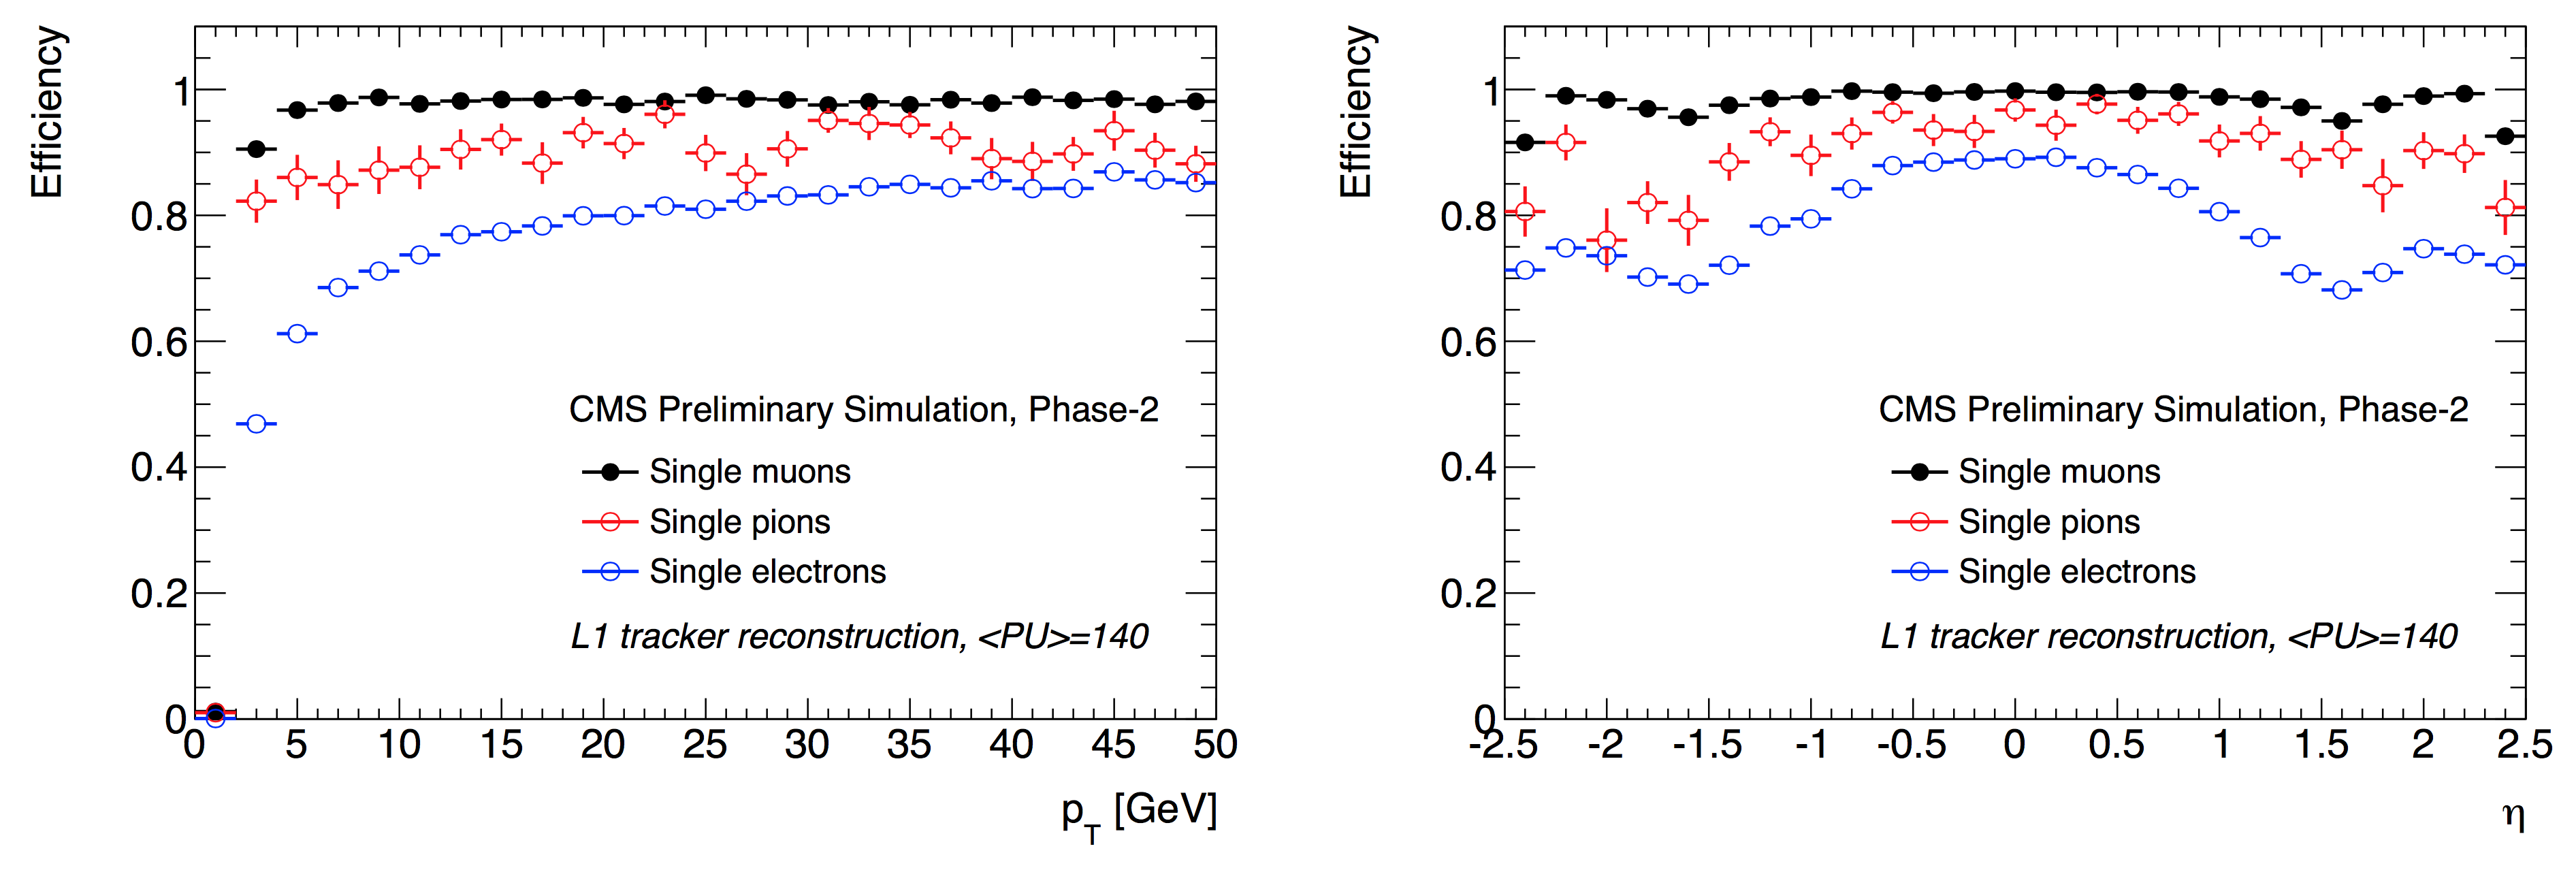
\includegraphics[width=\textwidth]{Figures/Efficiency.png}
	\caption{L1 track finding efficiency as a function of $p_T$ (left) and $\eta$ (right) for single muons, electrons, and pions with $p_T >$ 2 GeV and $|\eta| <$ 2.5 in events with $<$PU$>$=140.}
	\label{fig:Efficiency}
\end{figure}

\subsection{Resolutions}

The L1 track parameter resolutions are studied for single muons. Figure~\ref{fig:Resolution} shows, for three ranges of $p_T$, the estimated $z_0$ and relative $p_T$ resolutions as a function of $|\eta|$. Thanks to the PS modules the $z_0$ resolution is about 1 mm for a wide range of $\eta$, similar to the average separation of pileup vertexes, despite the large extrapolation distance (the first layer is at 25 cm). The relative $p_T$ resolution is about 1\% at central $\eta$ for high-$p_T$ tracks. The precise $z_0$ resolution is important to allow selecting tracks that originate from the same vertex for use in the trigger algorithms and the good $p_T$ resolution allows to have sharp muon trigger thresholds.
\begin{figure}[h!]
  \centering
	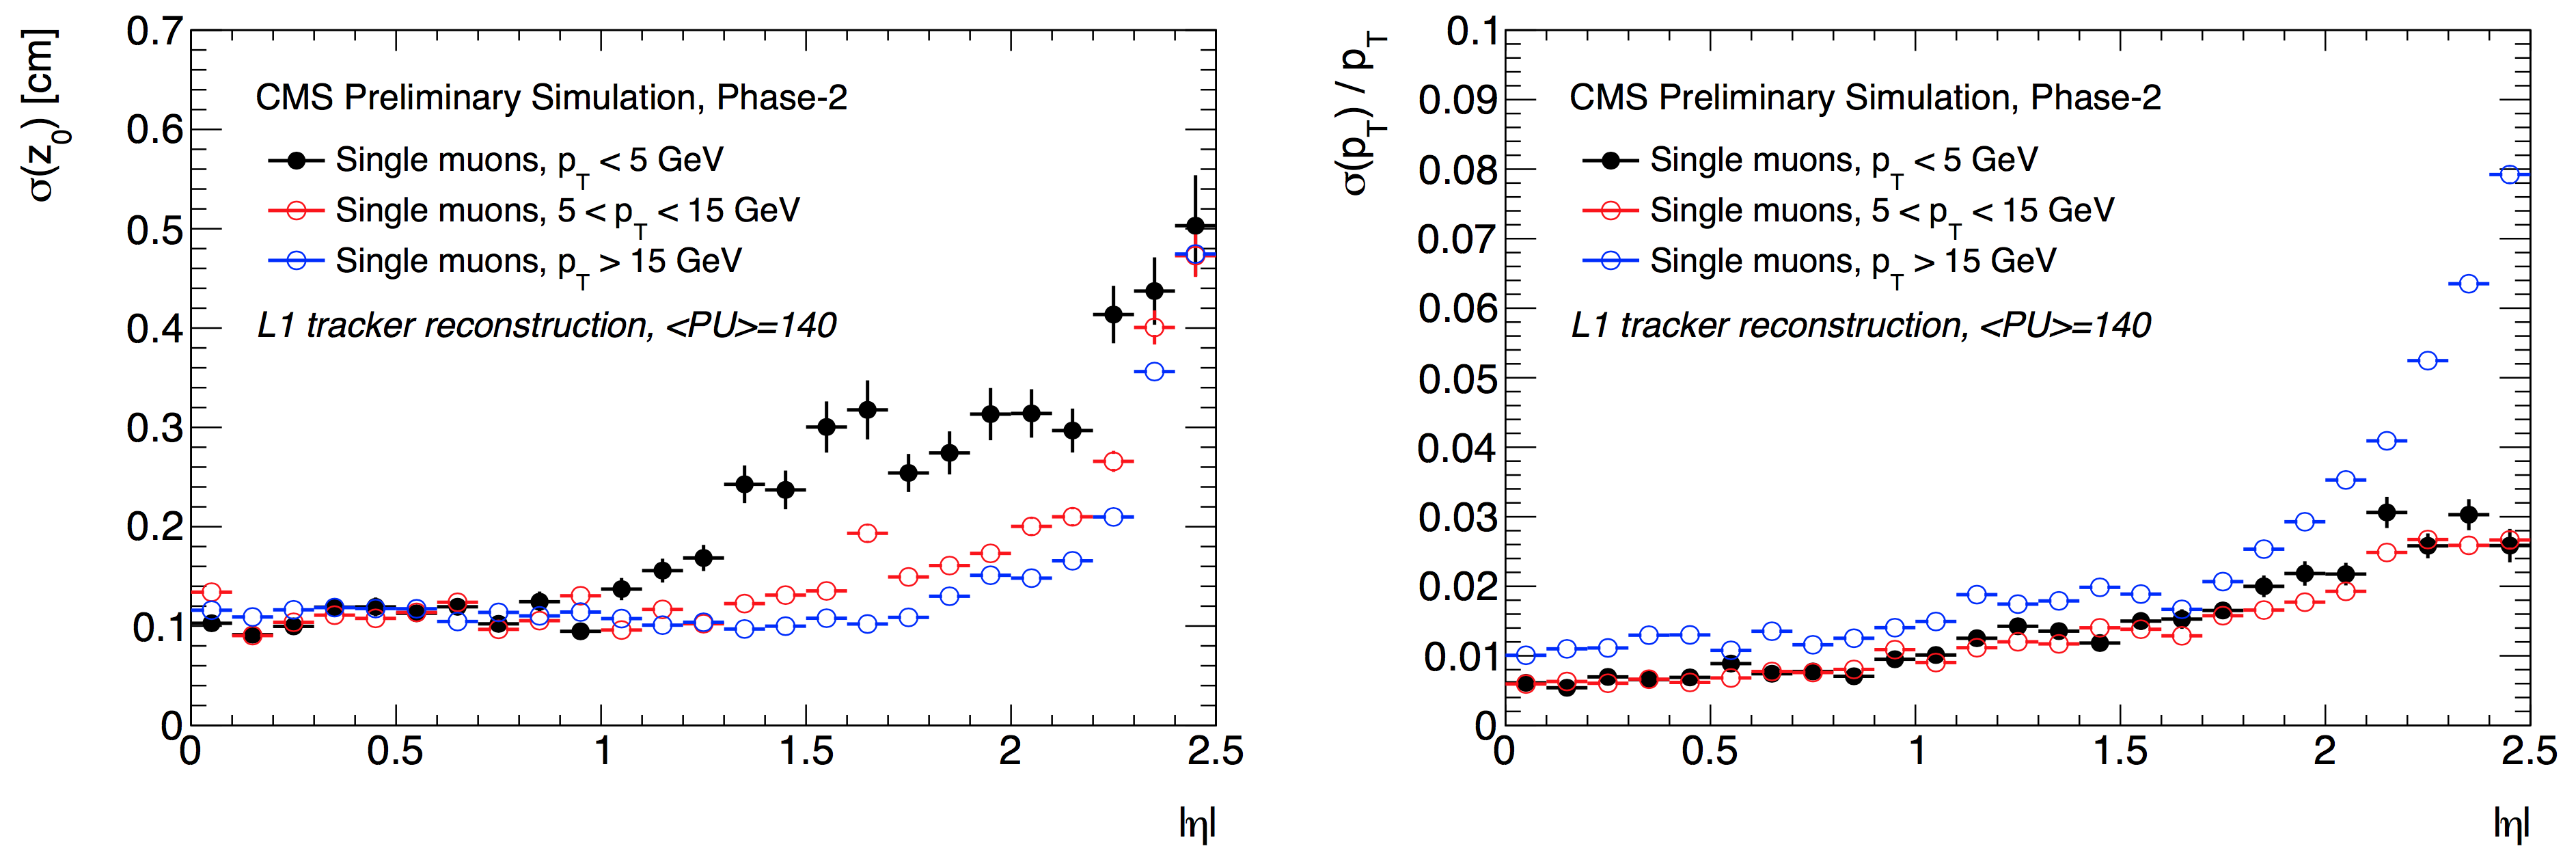
\includegraphics[width=\textwidth]{Figures/Resolution.png}
	\caption{Resolution of the L1 track $z_0$ (left) and relative $p_T$ (right) for single muons in events with $<$PU$>$=140. The resolutions are shown as a function of $|\eta|$ for three ranges of $p_T$.}
	\label{fig:Resolution}
\end{figure}

\section{Using L1 Tracks in the Trigger}

L1 trigger objects must be combined with L1 tracks to take advantage of L1 track information. This is done for leptons by matching L1 muon or calorimeter information with L1 tracks to derive improved muon momentum measurements or provide electron identification, to define track isolation variables, and to determine z positions for electrons, muons and taus. L1 tracks are also used to reconstruct the primary vertex of an event, and to perform vertex association for jets used in hadronic triggers.

\subsection{Lepton Triggers}

The trigger rates for single muons using the drift tube trigger primitives (DTTF)~\cite{DTTF} alone flatten as the threshold is increased. Matching DTTFs to L1 tracks can reduce this rate by a factor of 10 or more for $p_T$ thresholds above $\sim$14 GeV, as shown in Figure~\ref{fig:Rates} (left). For electrons, L1 $e/\gamma$ objects are matched to track stubs in the central region using either the current (5 $\times$ 5 crystal) L1 calorimeter granularity or single crystal-level position resolution~\cite{L1}. For a working point corresponding to 90\% signal efficiency, single $e/\gamma$ rates are reduced by a factor of $\sim$10 ($\sim$6) for signal (5 $\times$ 5) crystal granularity for $p_T > $ 20 GeV, as shown in Figure~\ref{fig:Rates} (right).
\begin{figure}[h!]
  \centering
	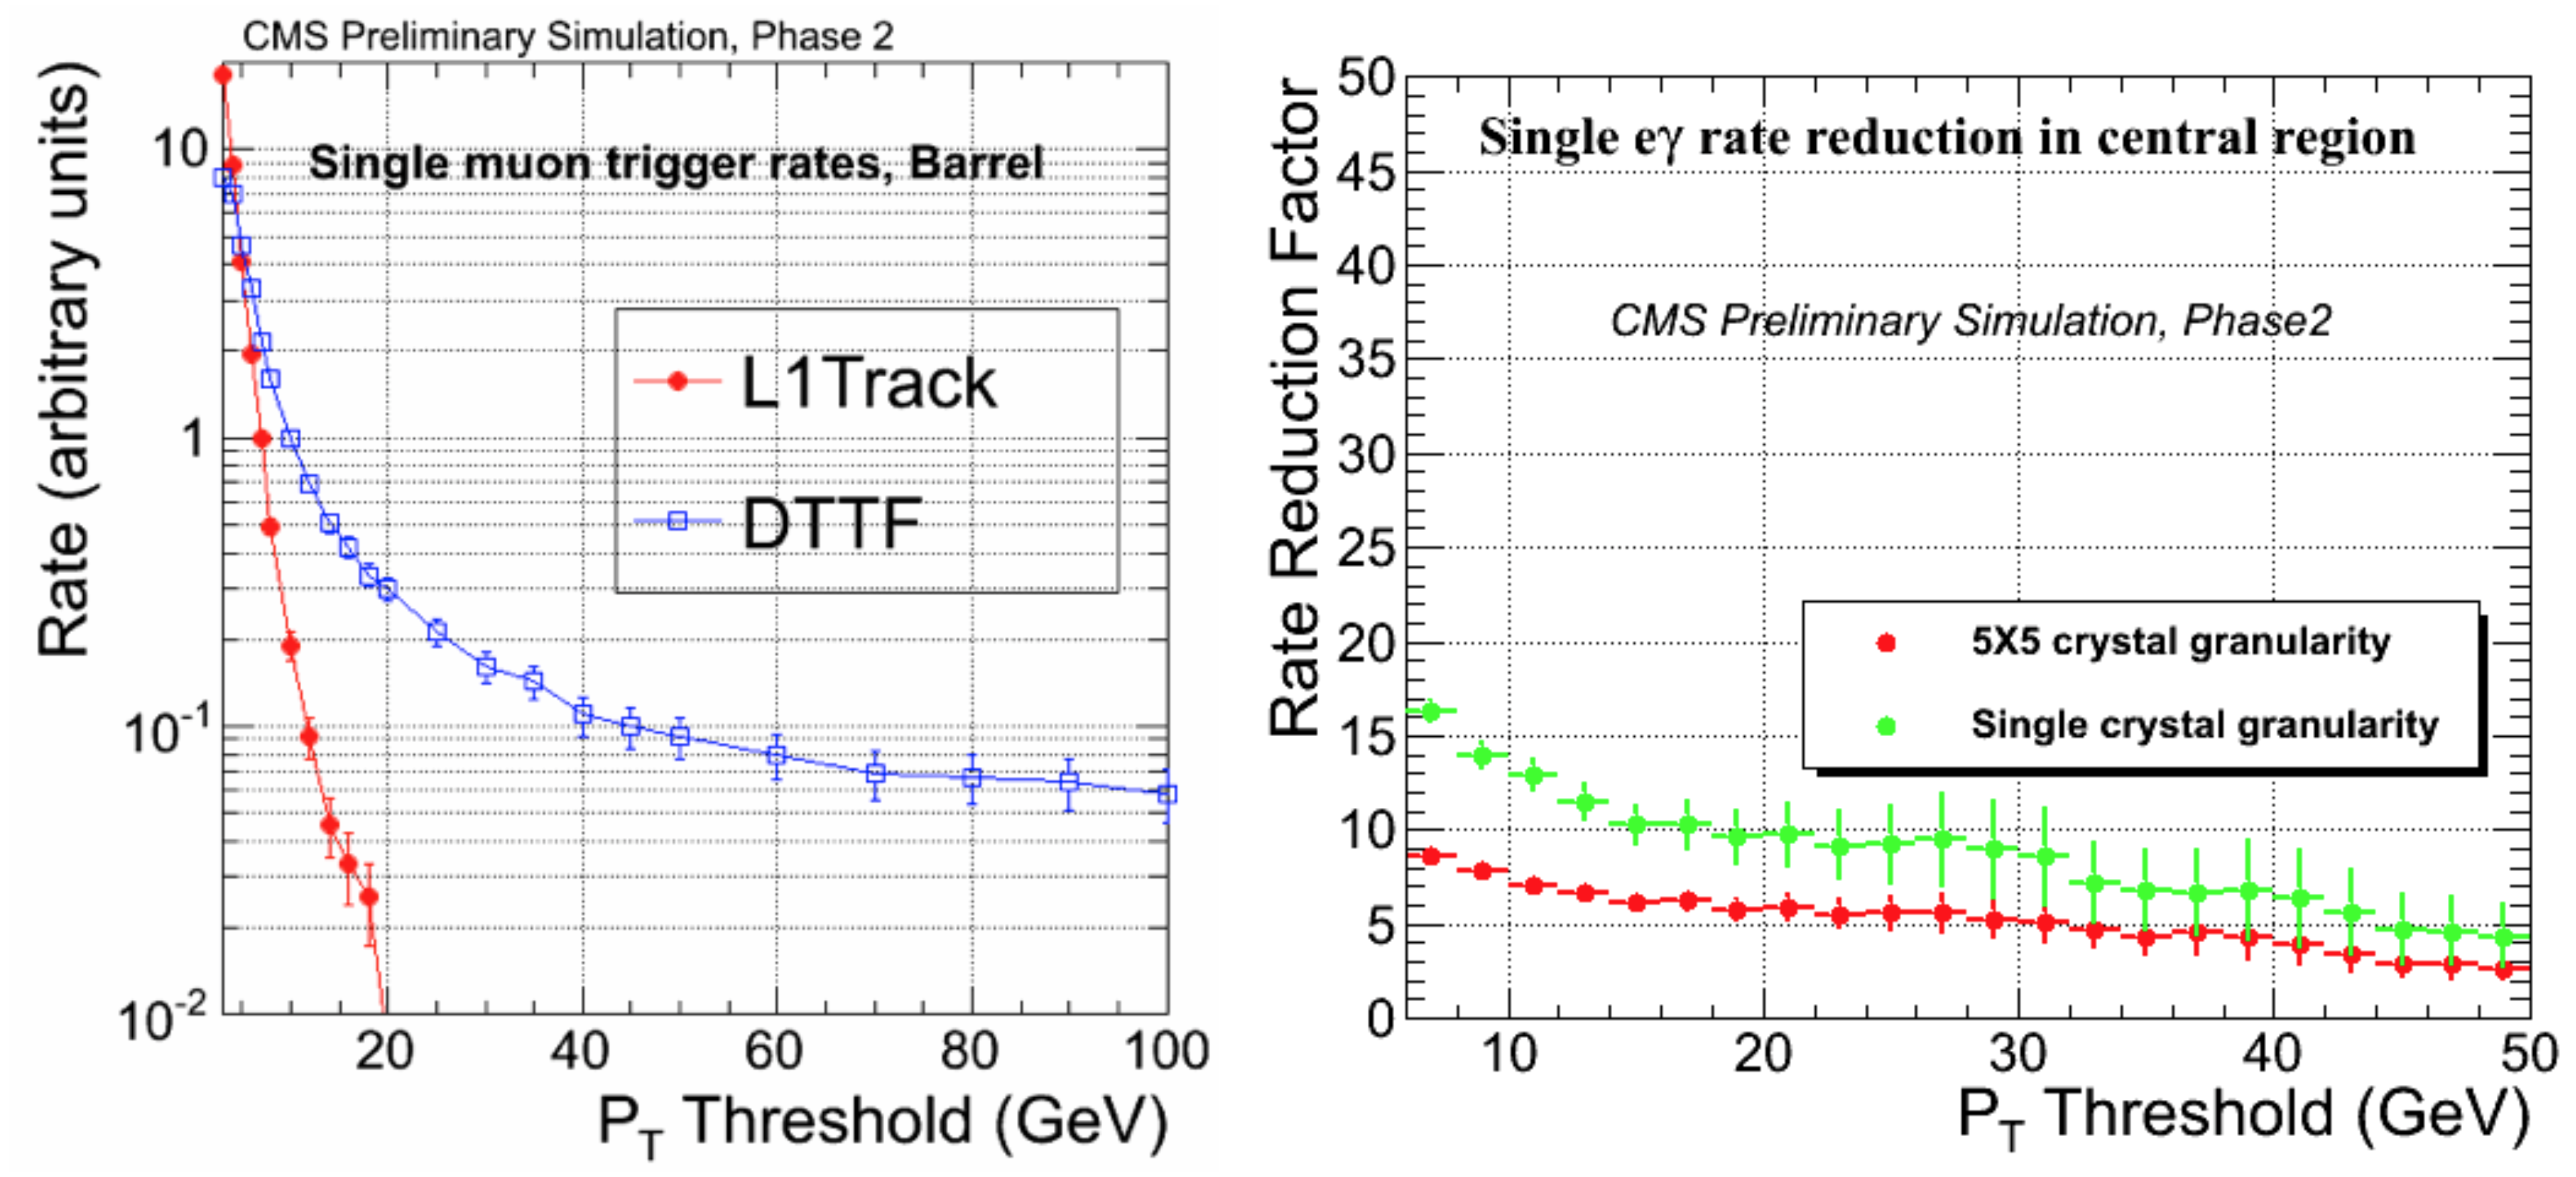
\includegraphics[width=\textwidth]{Figures/Rates.png}
	\caption{Single muon trigger rates for the barrel region normalized to the trigger utilized during Run 2 at 10 GeV (left) and single electron rate reductions, also for the central region, using single or (5 $\times$ 5) crystal granularity.}
	\label{fig:Rates}
\end{figure}

Lepton trigger rates can also be reduced via track-based isolation. As an example we consider a L1 $e/\gamma$ object with transverse energy $E_T$ and matched to a central L1 track. We define a relative isolation variable as $\sum p^{track}_T/E_T$, where the sum runs over tracks with $p_T >$ 2 GeV in an annulus of $0.02 < \Delta R < 0.2$ around the matched electron track\footnote{$\Delta R = \sqrt{\Delta\eta^2 + \Delta\phi^2}$, where $\Delta\eta (\Delta\phi)$ is the distance in $\eta (\phi)$ between the matched electron track and other tracks.}. The isolation variable is defined with or without requiring a $\delta z$ cut between the electron track and the tracks used for the isolation variable. Figure~\ref{fig:Isolation} shows the isolation efficiency for signal (single electron events with $<$PU$>$=140) versus background ($<$PU$>$=140 sample) for events in which a L1 track-electron candidate with $E_T >$ 20 GeV was found. A factor of two in rate reduction can be achieved for a 99\% signal efficiency when applying a $\delta z$ cut.
\begin{figure}[h!]
  \centering
	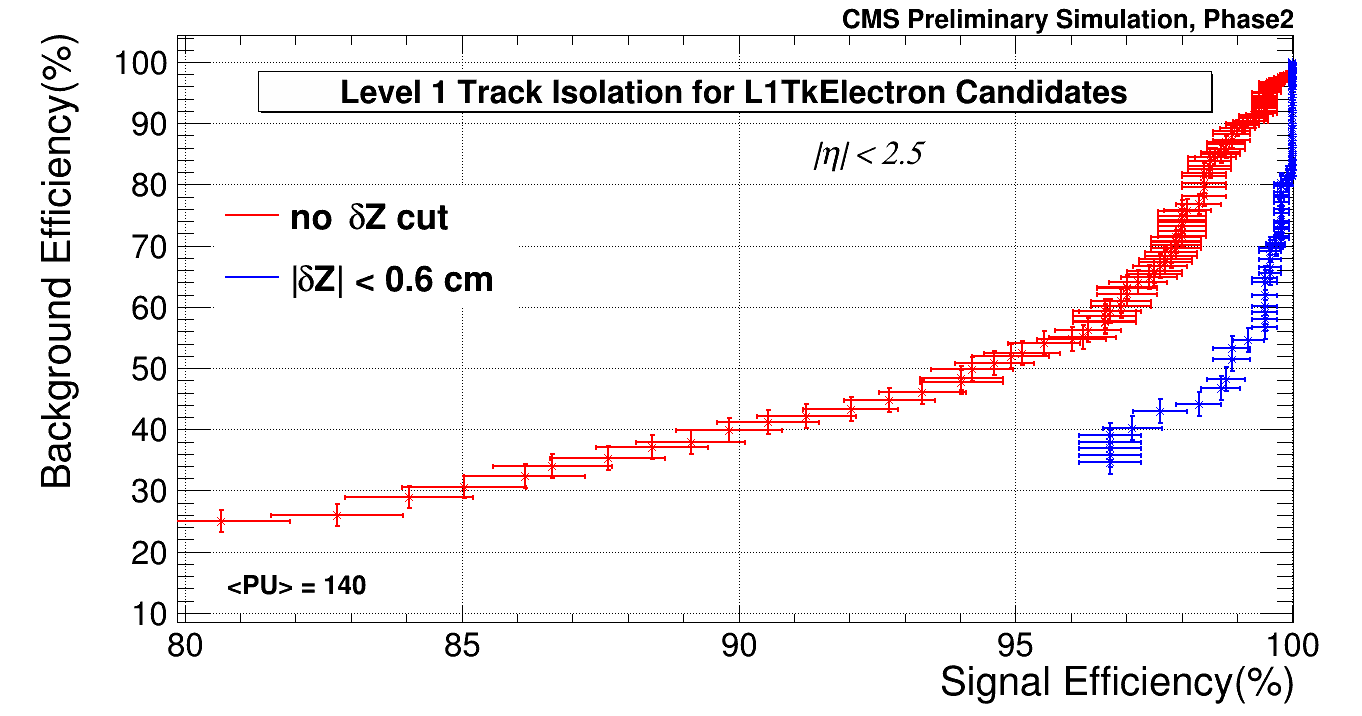
\includegraphics[width=0.5\textwidth]{Figures/isoROC_SignalEt20-25-4.png}
	\caption{Signal efficiency vs background efficiency for events in which a L1 electron object with $E_T >$ 20 GeV is found to be isolated with and without the $\delta z$ cut as described in the text.}
	\label{fig:Isolation}
\end{figure}

\subsection{Hadronic Triggers}
L1 track information can improve hadronic triggers by utilizing the tracks to measure jet z positions in jets and thereby be able to reject those coming from pileup interactions. The jet vertex is measured by associating the L1 jet object to nearby L1 tracks. The hadronic triggers can then select jets that originate from the same vertex through $\Delta z <$ 1 cm, defined in Figure~\ref{fig:JetDeltaZ}. For multijet triggers the requirement allows to utilize only the $n$ jets that are with $\Delta z <$ 1 cm with respect to the $z$ position of the leading jet.
\begin{figure}[h!]
  \centering
	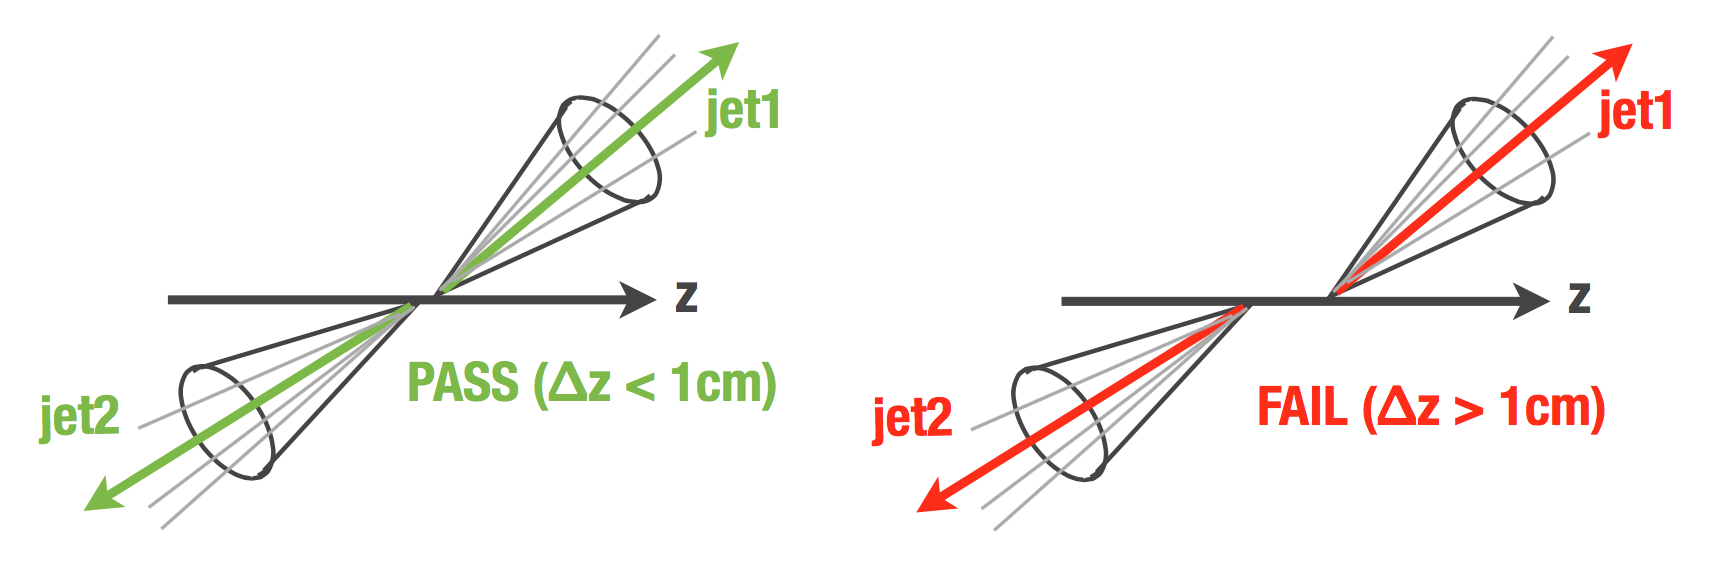
\includegraphics[width=0.5\textwidth]{Figures/JetDeltaZ.png}
	\caption{Vertex consistency requirement for hadronic triggers.}
	\label{fig:JetDeltaZ}
\end{figure}

To quantify the improvement in performance from the addition of L1 tracks, and in particular of vertex information, to the hadronic triggers we focus on two specific variables: $H_T$ and missing $E_T$, defined more precisely in the next paragraph. We define two kinds of $H_T$ triggers, with and without vertex association, as:
\begin{itemize}
\item No vertex association: $H_T = \sum p_T$(jet)
\item With vertex association: $H_T = \sum p_T$(jet) for jets with $|z$(jet)$ - z_{EVT}| <$ 1cm
\end{itemize}
where the sum is over jets with $p_T > 15$ GeV and $|\eta| <$ 2.0, and the event vertex $z_{EVT}$ is the $z$ position of the leading jet in the event. We define missing $H_T$ triggers In a similarly way with and without vertex association through the vector sum of the $p_T$ of jets.
The jet vertex performance is studied using all-hadronic $t\bar{t}$ events with $<$PU$>$=140. Figure~\ref{fig:JetVertex} (left) shows the efficiency of accurately measuring the jet $z$ position, defined as the efficiency of the cut $|z$(jet)$ - z_{true}| <$ 1 cm, as a function of the jet $p_T$. The efficiency is above 95\% for jets with $p_T >$ 50 GeV. Figure~\ref{fig:JetVertex} (right) shows the resolution of the measured $z$ position, which is about 1 mm.
\begin{figure}[h!]
  \centering
	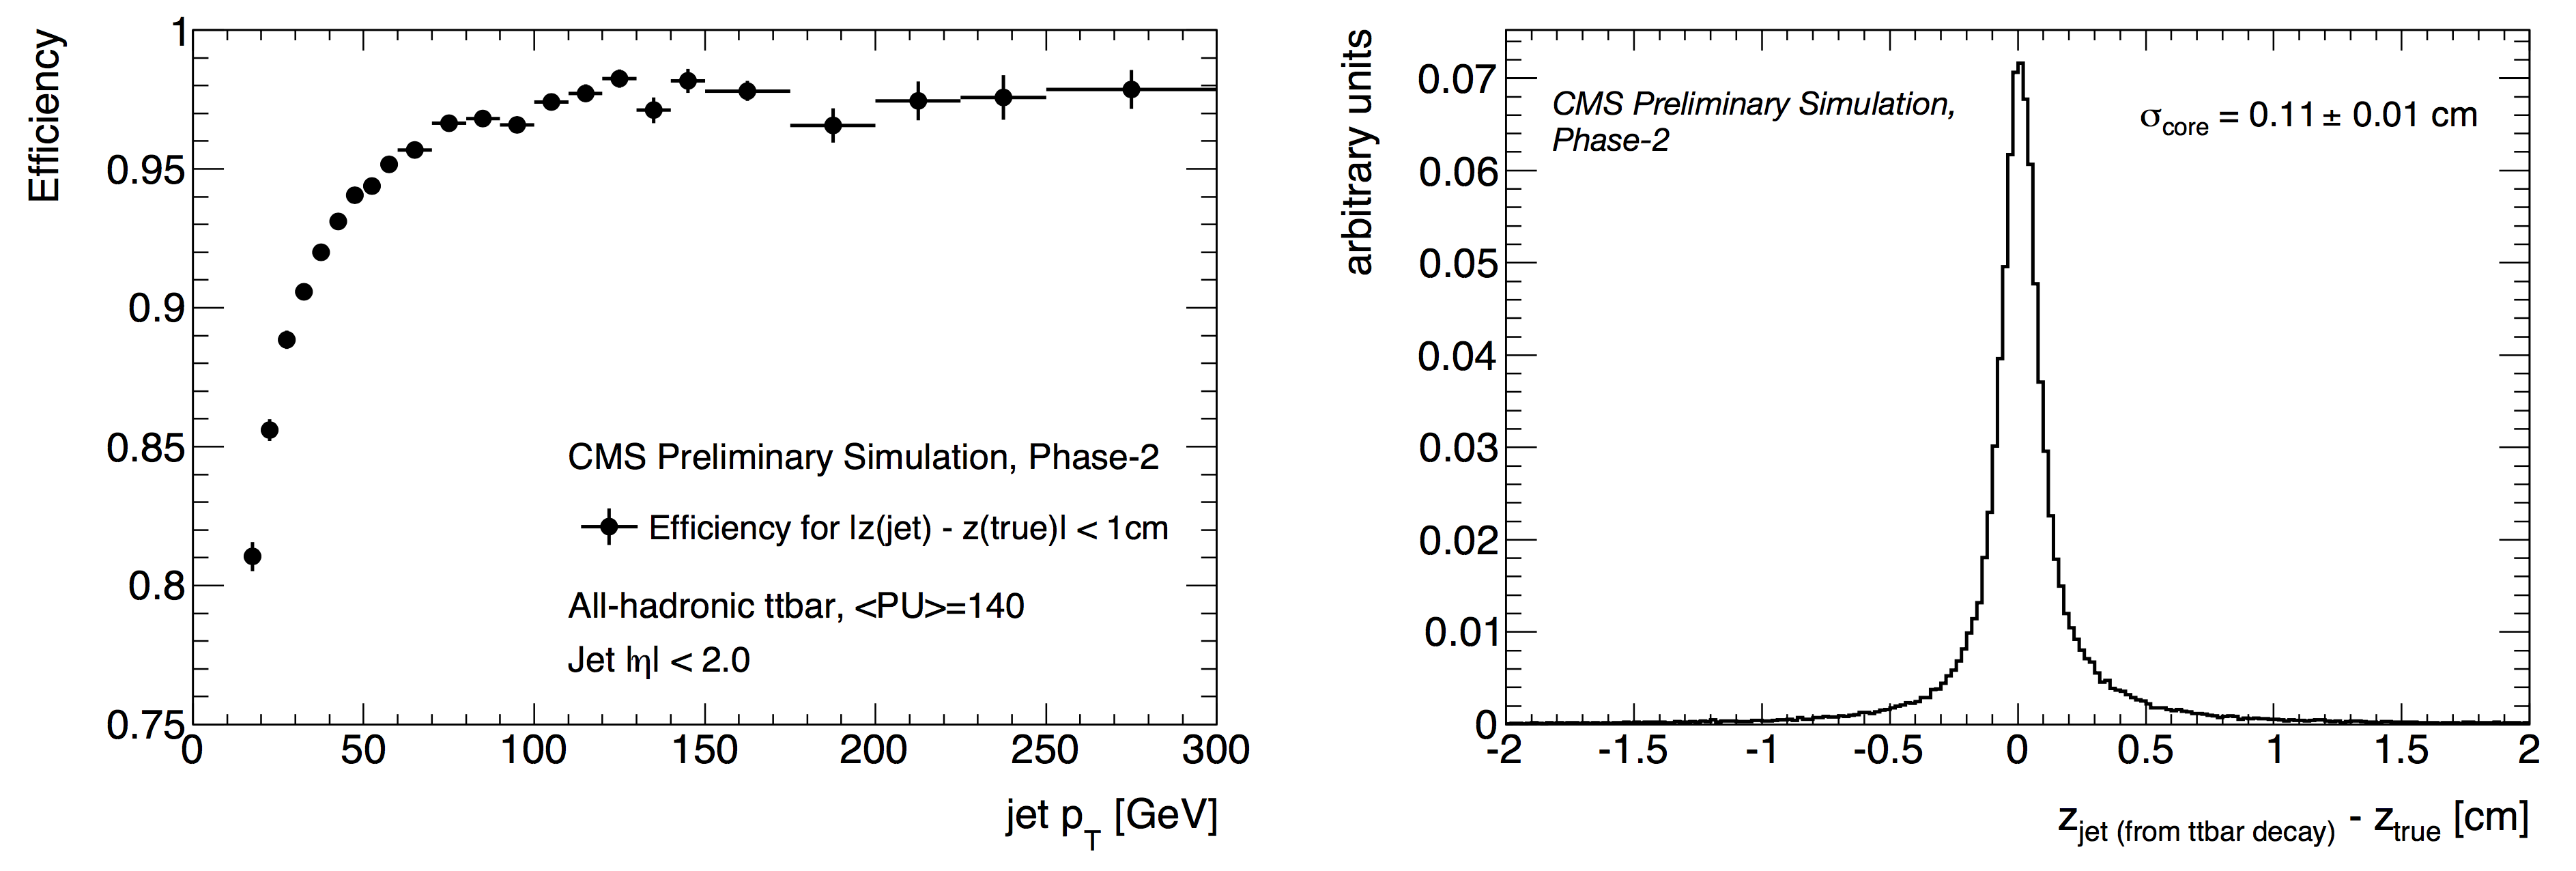
\includegraphics[width=\textwidth]{Figures/JetVertex.png}
	\caption{Efficiency to accurately measure the jet z position (left) and the resulting resolution (right), evaluated using all-hadronic $t\bar{t}$ events with $<$PU$>$=140.}
	\label{fig:JetVertex}
\end{figure}

An example supersymmetry signal point is utilized to assess the performance of including track information for hadronic triggers. The scenario 
considered is stop-quark pair production with hadronic top decays ($\tilde{t}\rightarrow t\tilde{\chi}^0_1$), where the stop mass is $m(\tilde{t})$ 
= 775 GeV and the neutralino mass $m(\tilde{\chi}^0_1)$ = 550 GeV. Figure~\ref{SUSY} shows the trigger rate versus signal efficiency for different missing
transverse energy and missing $H_T$ triggers: missing $E_T$ defined using calorimeter information only (CALOmet), missing $H_T$ determined 
with or without vertex association for two calorimeter-based L1 jet algorithms which differ in the PU subtraction methods used, and track-based 
missing transverse energy (TKmet). The track-based missing transverse energy variable is obtained utilizing L1 tracks coming from the primary 
vertex, where the primary vertex is also determined utilizing $z_0$ information from L1 tracks in the event. Significant rate reductions are achieved when incorporating L1 tracking information as shown in the figure.
\begin{figure}[h!]
  \centering
	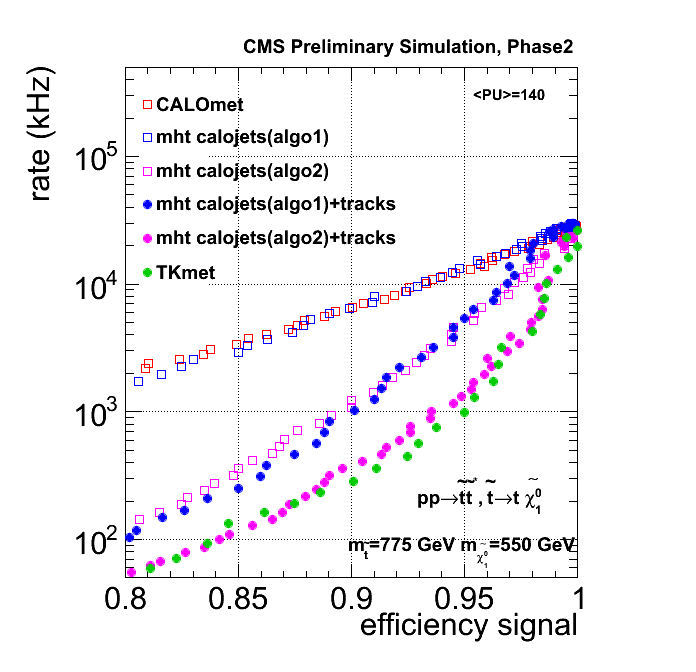
\includegraphics[width=0.5\textwidth]{Figures/roc_MHT_T2tt_775_550.png}
	\caption{Rate as a function of signal efficiency for inclusive missing transverse energy triggers for a supersymmetry scenario. The open symbols show the performance of triggers that do not make use of L1 tracking information with calorimetric missing $E_T$ and missing $H_T$ triggers. The filled symbols show the performance of triggers when adding L1 tracking information by constraining the jets used for missing $H_T$ triggers to originate from a common vertex or when defining a missing transverse energy variable utilizing L1 tracks originating from the primary vertex.}
	\label{fig:SUSY}
\end{figure}

\section{Conclusions}

As part of the upgrades for the HL-LHC, the CMS experiment plans to build a new tracker with triggering capabilities. This will allow to maintain high trigger efficiencies and to keep event rates at manageable levels without large increases in trigger thresholds. Three approaches to perform track reconstruction at the L1 trigger are being explored in parallel by the CMS collaboration. They rely on a combination of ASICs and commercial FPGAs for very low latency pattern matching and track fitting. These proceedings presented simulation studies of the performance of the L1 trigger including track information at CMS in the HL-LHC phase. The preliminary performance results are very promising, with high track-finding efficiency and precise measurements of L1 track parameters with about $\sigma(z_0)\sim$ 1 mm and $\sigma(p_T)/p_T \sim$ 1\% for a wide range of $\eta$.

The incorporation of L1 track information in the L1 trigger is driven by the physics requirements and it is important to achieve the necessary rate reductions. For electron and muon identification, rates can be reduced by a factor of $\sim$ 10. Adding track isolation gives another factor $\sim$ 2 in rate reduction. For hadronic triggers, large rate reductions can be achieved through determining the $z$ positions of jets and thereby requiring jets utilized for these triggers to originate from a common vertex.


\begin{thebibliography}{99}
\bibitem{SLHC} F. Zimmermann, \emph{CERN Upgrade Plans for the LHC and its Injectors}, CERN-sLHC-PROJECT-Report-0016 (2009).
\bibitem{CMS} The CMS Collaboration, \emph{The CMS experiment at the CERN LHC}, JINST 3 S08004 (2008), http://iopscience.iop.org/1748-0221/3/08/S08004/
\bibitem{CMSUpgrade} The CMS Collaboration, \emph{CMS Expression of Interest in the SLHC}, CERN/LHCC-2007-014, CERN (2007)
\bibitem{Tracklet} A. Ryd, \emph{CMS L1 Track Trigger for SLHC}, Contribution to Vertex 2009, 18th International Workshop on Vertex Detectors, Veluwe, the Netherlands, September 13Ð18 2009, PoS(VERTEX 2009)040
\bibitem{TkLayout} S. Mersi, G. Bianchi and S. Martina, The TkLayout Tool, http://mersi.web.cern.ch/mersi/layouts/.current
\bibitem{AM} F. Morsani et al., The AMchip: A VLSI associative memory for track finding, Nucl. Instrum. Meth. A 315 (1992) 446.
\bibitem{ATLAS_AM} A. Annovi et al., Associative Memory design for the fast track processor (FTK) at ATLAS, IEEE Nucl. Sci. Symp. Conf. Rec. (2011) 141.
\bibitem{DTTF} J. Erö et al, The CMS Drift Tube Trigger Track Finder, JINST 3 P08006 (2008), http://iopscience.iop.org/1748-0221/3/08/P08006/
\bibitem{L1} The CMS Collaboration, CMS Level-1 Trigger Technical Design Report, CERN/LHCC 2000-38, CMS TDR 6.1, CERN (2000)
\end{thebibliography}

\end{document}



\begin{document}

\section{...}
